%---------------------------------------------------------------------------
\documentclass[
	a4paper,				% paper format
	10pt,					% fontsize 
	oneside,				% double-sided
	parskip=half,		% set paragraph skip to half of a line
]{style}						% style class
%---------------------------------------------------------------------------

\def\matlab{{\em MatLab}}
\def\octave{{\em Octave}}

% === doc details ===
\def\mytitle{Solar System Simulation}
\def\mytitlepicture{imgs/example_small.jpg} % title imagecd
\def\titlepicturelength{1\textwidth} % width of the image
\def\untertitle{Simulation of our solar system}
\def\type{Applications of \matlab{}/\octave{}}
\def\myname{Eric Lochmatter, Lukas Studer}
\def\myfield{Micro- and Medicaltechnology}
\def\mydate{06. 01. 2016}
\def\myabstract{\matlab{} and \octave{} are very versatile programs. To explore the possibilities, we created a simulation of our solar system using \matlab{}. bla bla bla realism, bla bla bla to scale and some shit about not elipsies but circles}

% ------------------------------------------------------------------------

\begin{document}

\maketitle %title
\frontmatter
\tableofcontents\thispagestyle{toc}
\mainmatter


% === main content ===
\chapter{Introduction}
This project aims at creating a simple modle of our solar system using {\em MatLab.} While putting emphasis on the visuals, we kept the mathematical aspect simple.

Trajectories are not calculated and the orbits are perfect circles, due to the simple fact that the difference would be hardly noticeable. The sizes and distances are mostly to scale. We use a logarithmic scale for the sizes and a linear, though a very small scale, for the distances. 
\pagebreak
\chapter{Drawing the Planets and Orbits}
\section{Planets}
Drawing the planets is generally very simple: at first we create a sphere using the {\em sphere} function which gives us the coordinates {\em x}, {\em y} and {\em z} of each corner of the sphere while taking the  resolution as the argument. The resolution defines how smooth the surface of the sphere is. For example: a resolution of 50 generates a spheres composed of 50 equally wide rings with 50 equally big surfaces. Following images shows how the spheres react to different resolutions:

\begin{center}
\includegraphics[width=0.45\textwidth]{imgs/drawing_planets_orbits/spheres_res4.jpg}
\includegraphics[width=0.45\textwidth]{imgs/drawing_planets_orbits/spheres_res5.jpg}\\
\textit{Left: a sphere with resolution 4 (top and side view); Right: a sphere with resolution 5 (top and side view)}
\end{center}

We then manipulate the position values to scale and move the sphere as needed. We do this by multiplying the position matrices with a factor and then adding a constant to move it to the correct position.\\

Next we load the textures from an image using various \matlab{} functions: first we read the image of a map of the planet using {\em imread}. Then we convert the data to doubles using {\em im2double}. Next we use {\em imresize} to adjust the image the size of the planet. We then only have to flip the data upside down to correctly display the texture. This is done using the {\em flipud} function. Further details for these function can be found in the help pages of each function.\\

Last but no least we create a surface object, or the 'planet', using the {\em surf} function by passing the position matrices and the textures. We can then use this object to move and rotated the planet.

Following {\em MatLab} code draws a simple sphere with a texture as described above:
\begin{framed}\begin{verbatim}
[x,y,z] = sphere(resolution);
x = x*scale(1) + pos(1); y = y*scale(2) + pos(2); z = z*scale(3) + pos(3);

texture = flipud(imresize(im2double(imread(imgFile)),size(x)));
planet = surf(x, y, z, texture,'EdgeColor', 'none');
\end{verbatim}\end{framed}
{\em pos} and {\em scale} are vectors containing the coordinates of the center of the planet and factors for stretching the planet in {\em x}, {\em y} and {\em z} directions. {\em imgFile} is a string containing the path to the textures of the planet and {\em resolution} is an integer for the resolution of the sphere as described above.

\subsection{Rings}
Some planets, in our case only saturn, have rings of water ice and rocky material circling them. To respect the thickness of such rings and for simplicity we created them using a torus and squished it to make it thiner. A torus is described as follows:

\begin{align*}
x(\theta, \varphi) = (R + r*\cos(\theta) * \cos(\varphi)\\
y(\theta, \varphi) = (R + r*\cos(\theta) * \sin(\varphi)\\
x(\theta, \varphi) = r*\sin(\varphi)
\end{align*}

$\theta$, $\varphi$ are angles which make a full circle, so that their values start and end at the same point,\\
R is the distance from the center of the tube to the center of the torus,\\
r is the radius of the tube.

In \matlab{} this looks some what like this:
\begin{framed}\begin{verbatim}
phi = linspace(0,2*pi,resolution)';
alpha = linspace(0,2*pi,resolution*10)';

tmp = [R + r*cos(phi), r*sin(phi)];
x = cos(alpha)*tmp(:,1)';
y = sin(alpha)*tmp(:,1)';
z = tmp(:,2)';
z = z(ones(1,length(alpha)),:);
\end{verbatim}\end{framed}
The rest for drawing the ring is the same as for drawing the planets: we move and scale the ring using vectors containing the position of the center and factors for each direction and then create a surface object with the textures of the ring. Only the textures are slightly different compared to the planets. While the planets use a map, the ring has to be only a portion of the ring mirrored along the inner {\em 'edge'} of the ring.


\section{\textcolor{red}{Orbits}}
Drawing the trajectory of the planets was made a lot easier when we decided to use circles as orbits instead of calculating them.

\begin{framed}\begin{verbatim}
theta = 0:0.01:(2*pi+0.01);
v = null(normal);
points = repmat(center',1,size(theta,2))+radius*(v(:,1)*cos(theta)+v(:,2)*sin(theta));
orbit = plot3(points(1,:),points(2,:),points(3,:),'Color',color);
\end{verbatim}\end{framed}

\pagebreak
\section{Key Values for the Modle}
As said before, we tryed to use realistic values and scales for the modle. Listed in the following two chapters are the values we ended up using.

\subsection{Distances}
\begin{center}
    \begin{tabular}{| l | l | l | l |}
    \hline
    Planet & Distance [km] & Distance [AU] & Scale Factor \\ \hline
    Mercury & 57'909'227 & 0.39 & 0.39 \\ \hline
    Venus & 108'209'475 & 0.73 & 0.73 \\ \hline
    Earth & 149'598'262 & 1 & 1 \\ \hline
    Moon & 384'400 & 0.0025 & 0.0025 \\ \hline
    Mars & 227'943'824 & 1.38 & 1.38 \\ \hline
    Jupiter & 778'340'821 & 5.20 & 5.20 \\ \hline
    Saturn & 1'426'666'422 & 9.58 & 9.58 \\ \hline
    Uranus & 2'870'658'186 & 19.22 & 19.22 \\ \hline
    Neptune & 4'498'396'441 & 30.10 & 30.10 \\
    \hline
    \end{tabular}\\
    \textit{The distances are all the average distance from the sun.\\
    Except for the moon, whose distance is the average distance from earth.}
\end{center}


\subsection{Sizes}
\begin{center}
    \begin{tabular}{| l | l | l |}
    \hline
    Planet & Diameter [km] & Scale Factor \\ \hline
    Sun & 1'392'684 & 109.18 \\ \hline
    Mercury & 4'879 & 0.38 \\ \hline
    Venus & 12'104 & 0.95 \\ \hline
    Earth & 12'756 & 1 \\ \hline
    Moon & 3'475 & 0.27 \\ \hline
    Mars & 6'805 & 0.53 \\ \hline
    Jupiter & 142'984 & 11.21 \\ \hline
    Saturn & 120'536 & 9.45 \\ \hline
    Uranus & 51'118 & 4.01 \\ \hline
    Neptune & 49'528 & 3.88 \\
    \hline
    \end{tabular}\\
    \textit{The diameters used are the equatorial diameters of the planets.\\
    The scale factor used is log10 of the value in this table.}
\end{center}


\subsection{Speed}
\begin{center}
    \begin{tabular}{| l | l | l |}
    \hline
    Planet & Earth days / year & Scale Factor \\ \hline
    Mercury & 87.97 & 4.1521 \\ \hline
    Venus & 224.7 & 1.6255 \\ \hline
    Earth & 365.26 & 1 \\ \hline
    Moon & 27.3 & 13.3795 \\ \hline
    Mars & 686.98 & 0.5317 \\ \hline
    Jupiter & 4332.82 & 0.0843 \\ \hline
    Saturn & 10755.7 & 0.034 \\ \hline
    Uranus & 30687.15 & 0.0119 \\ \hline
    Neptune & 60190.03 & 0.0061 \\
    \hline
    \end{tabular}\\
    \textit{The scale factor is used for the orbit speed.\\
    Therefor less days mean faster orbit speed.}
\end{center}

\chapter{Moving the Planets}
The decision to use circular orbits also influenced how we moved the planets in out modle. We were able to use the {\em rotate} function from \matlab{}. This function allows us to rotate the objects by a number of degrees around a vector at a given position. Due to the flexibility, we can use this function for all the movement in the modle. This includes the movement along the orbit, the spin of planets and keeping the rotation axis of planets aligned.\\

To animate the modle, we move all objects using the {\em rotate} function and then refresh the graph. We defined this to be one tick. This way of animating the modle may be very simple, but proved to have some unpleasant side effects as described below.

\section{Earth's Spin}
We defined the {\em 'normal'} speed of the modle to be so that the earth rotates one degree around the sun per tick. This means that it takes earth 360 ticks to complete one year's worth of rotation. This on the other hand means that, rounding the number for this explanation, earth has to rotate once around itself per tick. This would result in, again rounding the numbers, 365 earth days per earth year which, as we all know, would be correct. Using the {\em rotate} function to rotate earth 360 degrees around itself per tick, results in no visible spin of earth. Using the real numbers would still result in only a very slow spin, due to the fact that it rotates a bit more than 360 degrees per tick\\

We {\em solved} this problem by giving earth an arbitrary speed of rotation around itself.


\section{Increased Speed}
Basically the same problem occurs when increasing the speed of the animation using the slider. As described in the chapter {\em UI Elements}, the slider only increases the angle of rotation. Setting the speed to higher values leads to visual effects similar to those of aliasing. The basic principle of aliasing is that the sample rate of the measuring device is to slow for what it is measuring, which leads to distorted results. In our case, we generate to few steps to create a smooth animation. This makes planets jump, rather than smoothly move, and rotate clockwise rather than counter clockwise. As a simple example, if  the rotation angle is set to 90 degrees earth would jump three times before returning to its starting position. This is drastically different to the 360 steps earth makes at normal speed. \\

As already the one above, we weren't able to fix the problem and could only restrict the maximum speed, which works for the planets in the outer solar system but not so much for the planets closer to the sun.
\chapter{UI Elements}

The modle provides two UI elements for the user, besides the common controls from {\em MatLab} itself. A display for the number of frames rendered pre second and a slider to control the speed at which the modle runs.

\section{FPS Display}
While programing the modle we soon realized that the certain changes had a massive impact on the number of frames {\em MatLab} could render per second. The number of frames per second, also known as {\em FPS} directally dictates how smooth the modle runs. Through time analysis of the modle we found out that the resolution of the planets, sun, and moon had the most noticable impact on the {\em FPS.} We then added the display to find the optimal resolution at which the graphics of the planets didn't suffer to much but still allowed for a smooth animation. We settled for a resolution of 50. This generates spheres composed of 50 equally wide rings with 50 equally big surfaces. This keeps the {\em FPS} around 20 which is only slightly lower than the number images the human eye can capture per secend. This makes the animation appear smooth. Following images shows how the sphreres react to different resolutions:

\begin{center}
\includegraphics[width=0.45\textwidth]{imgs/ui_elements/spheres_res4.jpg}
\includegraphics[width=0.45\textwidth]{imgs/ui_elements/spheres_res5.jpg}\\
\textit{Left: a sphere with resolution 4 (top and side view); Right: a sphere with resolution 5 (top and side view)}
\end{center}

\textcolor{red}{CALCULATION OF FPS}

\section{Speed Slider}
Because Uranus and Neptune are so far away from the sun, it takes them quite a while to complete an entire turn around the sun. That is why we added a slider on the bottom left which allows users to speed up the animation. Additionally the slider can also stop the animation by setting the speed to zero which allows for closer inspection of the planets. The slider basically controls the angle of rotation per tick. Faster speed results in a grater angle. Setting the speed to higher values leads to visual effects like planets appearing to jump rather than smoothly moving and planets smoothfully to be turning backwards. Alternatives like controling a delay for rendering the next frame have been tested, but didn't work out due to the {\em FPS} plummeting or the animation quickly reaching a maximum speed and therefore not having the desired effect.

\chapter{Appendix}
\section{Code}
\subsection{FILENAME}


\end{document}